\documentclass[a4paper]{article}
\usepackage[margin=3cm]{geometry}
\usepackage[utf8]{inputenc}
\usepackage{cmbright}
\usepackage[hidelinks]{hyperref}
\usepackage{booktabs}
\usepackage[ngerman]{babel}
\usepackage{parskip}
\usepackage{graphicx}
\usepackage{minted}
\usepackage{pdflscape}
\usepackage{array}
\usepackage{tabulary}
\usepackage{multicol}
\usepackage{pgfgantt}
\usepackage{pgf-umlcd}
\usepackage{enumitem}

% Page breaks between sections
\let\oldsection\section
\renewcommand\section{\clearpage\oldsection}

% JIRA/Confluence shortcuts
\def\jiraurl{https://jira.keltec.ch/jira}
\def\confluenceurl{https://jira.keltec.ch/wiki}
\newcommand{\jiraissue}[1]{\href{\jiraurl/projects/EPJ/issues/EPJ-#1}{EPJ-#1}}
\newcommand{\fulljiraissue}[1]{EPJ-#1 (\url{\jiraurl/projects/EPJ/issues/EPJ-#1})}

% Tools
\newcommand{\tool}[2]{\emph{#1\footnote{\url{#2}}}}

\begin{document}
	\title{
		Projekt: kitovu \\
		\Large{Softwarearchitektur} \\[3em]
		
\includegraphics[width=20em]{../../img/logo/kitovu.jpg}
	}
	\author{
		Florian Bruhin \\ \url{florian.bruhin@hsr.ch} \and
		Méline Sieber \\ \url{meline.sieber@hsr.ch} \and
		Nicolas Ganz \\ \url{nicolas.ganz@hsr.ch} 
		}
	\date{\today}
	
	\maketitle

\section*{Änderungsgeschichte}

\begin{tabulary}{\linewidth}{llLl}
	\toprule
	Datum & Version & Änderung & AutorIn \\
	\midrule
	28.03.2018 & 1.0 & Dokument erstellt, Grundgerüst von Template übernommen & Méline Sieber \\

	\bottomrule
\end{tabulary}
\pagebreak

\section{Einführung}
Dieses Dokument schliesst die Entwicklungsphase ``End of Elaboration'' ab. Es legt dar, wie die Software-Architektur von \emph{kitovu} aufgebaut ist, beschreibt die logischen Schichten und deren Zusammenhänge. Zudem klärt es die grössten Risiken des Projekts, namentlich die Einbindung der beiden externen Plattformen (Studentenportal, Moodle). Das Dokument erläutert auch die Herausforderung, die grafische Benutzeroberfläche mit dem Kommandozeilen-Client zu verbinden (Prozesse und Threads). Als letzter Punkt wird der Aspekt der Datenspeicherung, insbesondere der Aufbau der Konfigurationsdatei besprochen.

Es bleibt eine Anmerkung: Viele Punkte der ``End of Elaboration'' definiert schon der sehr ausführliche Projektplan. Um das dieses Dokument möglichst schlank zu halten, werden deshalb gewisse Punkte aussen vor gelassen, insbesondere die Ausführungen zur Grösse und Leistung von \emph{kitovu}.

\subsection{Gültigkeitsbereich}
Die vorliegende Architekturbeschreibung ist für das Engineering-Projekt im Frühlingssemester 2018 gültig. Falls dem Projekt grössere Veränderungen widerfahren, wird das Dokument dementsprechend angepasst. Umfassende Änderungen werden am Anfang des Dokuments protokolliert.

\subsection{Referenzen}
Die Anforderungsspezifikation ist eng mit der Domainanalyse und anderen Dokumenten verbunden. Die folgende Tabelle listet die wichtigsten Referenzen auf.

\begin{tabulary}{\linewidth}{Ll}
	Confluence & \url{\confluenceurl} \\
	Draw.io & \url{https://www.draw.io/} \\
	Github-Repository von \emph{kitovu} & \url{https://github.com/kitovu-bot/kitovu} \\
	JIRA	& \url{\jiraurl} \\
	Moodle & \url{https://moodle.hsr.ch} \\
	OpenHSR Connect & \url{https://github.com/openhsr/connect} \\
	Studentenportal & \url{https://studentenportal.ch/} \\
	Switch AAI \newline (Authentication and Authorization Infrastructure)& \url{https://www.switch.ch/aai/} \\
\end{tabulary}

Beim Logo auf der Titelseite handelt es sich um eine stark überarbeitete Version eines GIFs (\url{https://www.animateit.net/details.php?image_id=8990}). Urheber und Copyright sind nicht auffindbar.

\pagebreak

\section{Systemübersicht}

Das folgende Kontextprogramm verdeutlicht, wie die Schnittstellen von \emph{kitovu} aussehen. Auf der einen Seite  sind die Nutzerinnen und Nutzer, die je nach Informatikkenntnissen mit der grafischen Oberfläche oder mit dem Kommandozeilenprogramm interagieren. Auf der andere Seite sind die Plattformen, die \emph{kitovu} einbindet: Der Skripteserver sowie die Moodle-Plattform, die jedoch eine Authentifikation via Switch AAI verlangt. Weshalb das Studentenportal für dieses Projekt nicht implementiert werden kann, erklärt der nächste Abschnitt.

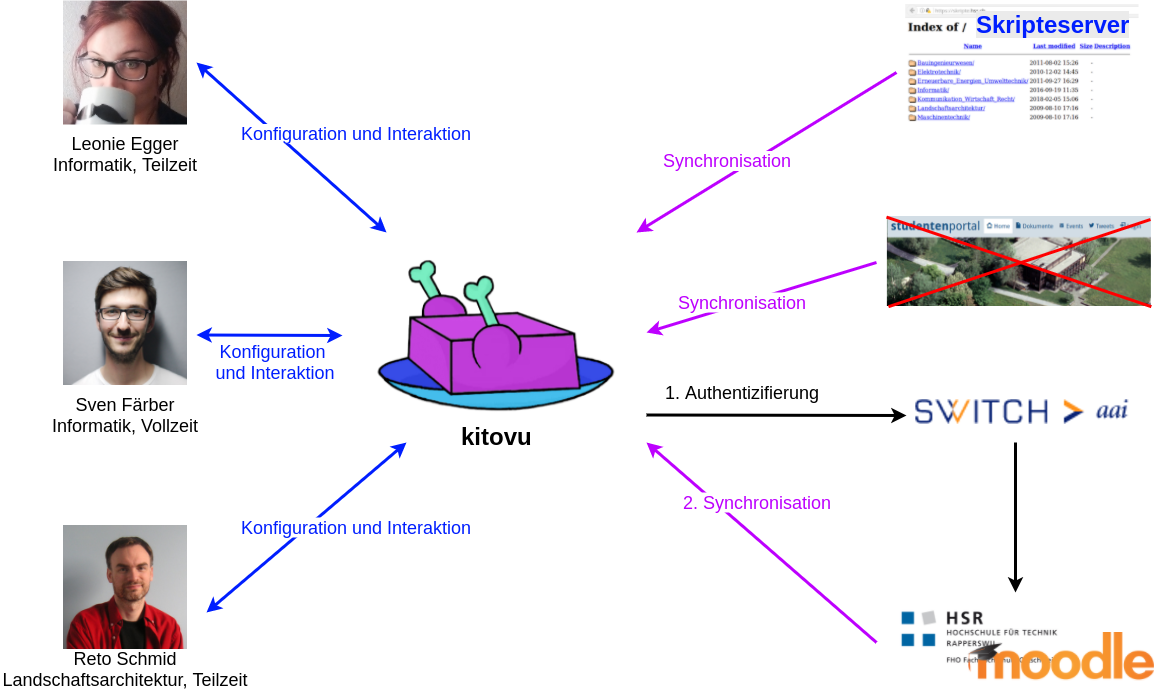
\includegraphics[width=40em]{./img/kontextdiagramm.png}

% <Beschreibt die Softwarearchitektur eines Systems und wie sie sich präsentiert (am besten mit einem Bild um eine Übersicht zu ermöglichen) und einzelne Beschreibungen zu den einzelnen Elementen des Systems>



\section{Architektonische Ziele und Einschränkungen}

Der Projektplan erläuterte bereits die beiden grössten Risiken: Die Einbindung des Studentenportals und von Moodle, so dass sich von beiden Plattformen auch Dokumente synchronisieren lassen.

Zum Ende der Elaborationsphase zeigt sich nun, dass sich diese frühzeitige Einschränkung des Projekts gelohnt hat: Die Abklärung mit dem OpenHSR-Verein und den Betreibern des Studentenportals ergab, dass wir darauf verzichten müssen, das Portal einzubinden. Es fehlt an einer API, mit der wir Files synchronisieren könnten -- wir müssten dies von Hand hinzufügen, was den Rahmen des Projekts sprengt. Zudem sind viele Komponente des Studentenportals veraltet und sollten dringend aktualisiert werden. Ein möglicher Sprint sollte dem Abhilfe schaffen. Doch diesen organisiert die Fachschaft oder der OpenHSR-Verein und ist somit ausserhalb unseres Projekts. Das Studentenportal wird somit kein Teil von \emph{kitovu}.

Das zweite Risiko, die Moodle-Einbindung, ist noch in weiterer Abklärung, aber es bestätigt sich ebenfalls die erste Einschätzung: Die Einbindung wird nicht einfach. Zum einen ist die WebDAV-Schnittstelle schon älter -- wenn nicht gar veraltet --, zum anderen fehlen noch wichtige Informationen, etwa die aktuellste Dokumentation zum Moodle-Desktop-Client. Da Moodle eine wichtige Unterrichtskomponente ist, werden wir die Einbindung versuchen, soweit es unsere Kapazitäten zulassen. Die Plattform ist jedoch immer noch optional für das Gelingen des Projekts.

\section{Logische Architektur}

% <Beschreibung der logischen Struktur des Projekts. Pro Subsystem/Package ein einzelner Abschnitt und ein Übersichtsdiagramm über die einzelnen Subsysteme/Packages. Aufteilung in Subsysteme/Packages (zum Beispiel: 3-Layer-Architektur mit GUI, Problem Domain und Datenhaltung). >

% Weitere Punkte: Klassenstruktur, Schnittstellen, Wichtige interne Abläufe, Wichtige Abläufe

\subsection{Schichten}

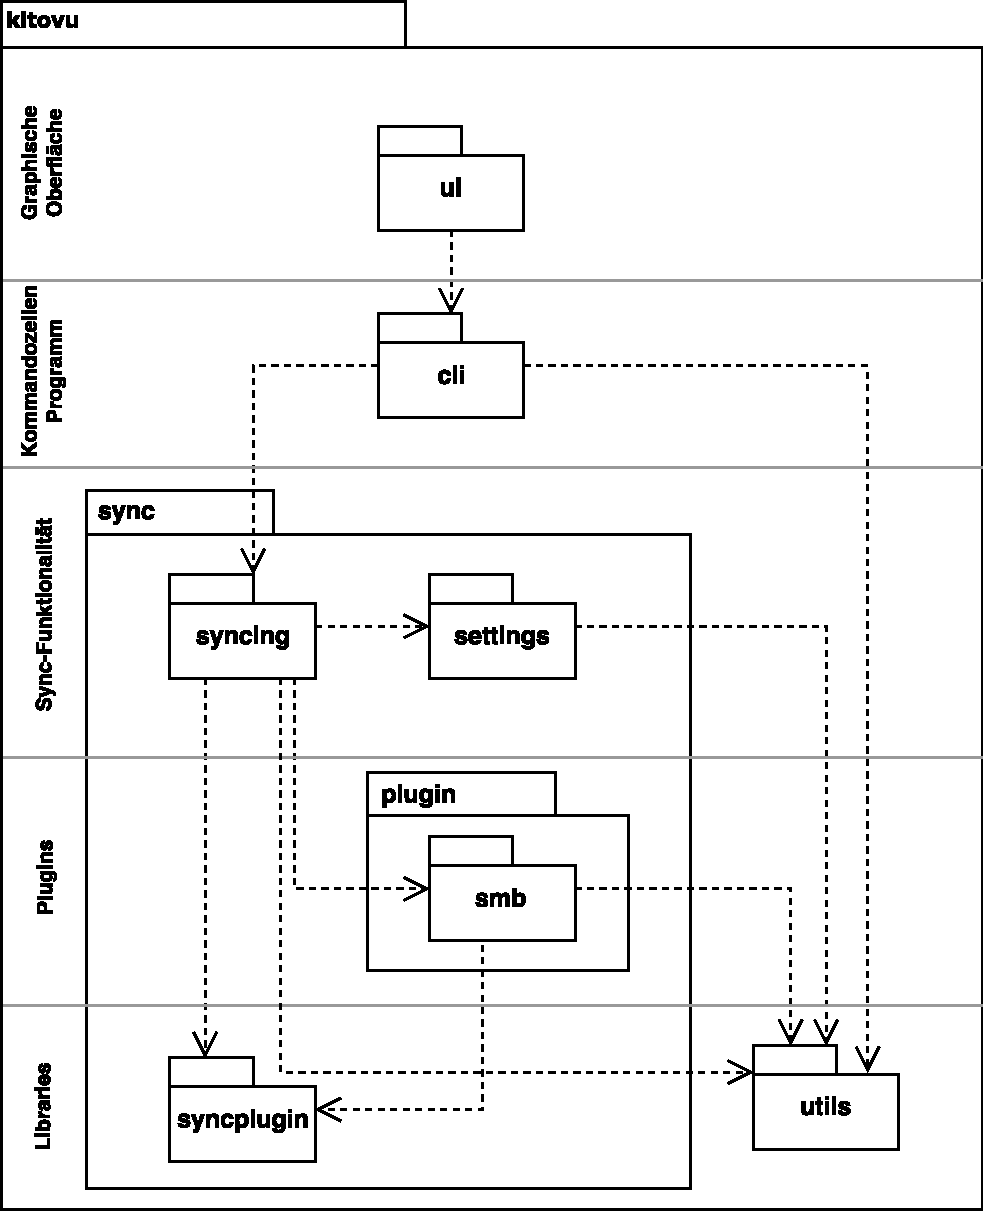
\includegraphics[width=40em]{./img/schichtendiagramm.pdf}

\subsection{Sequenzdiagramm}

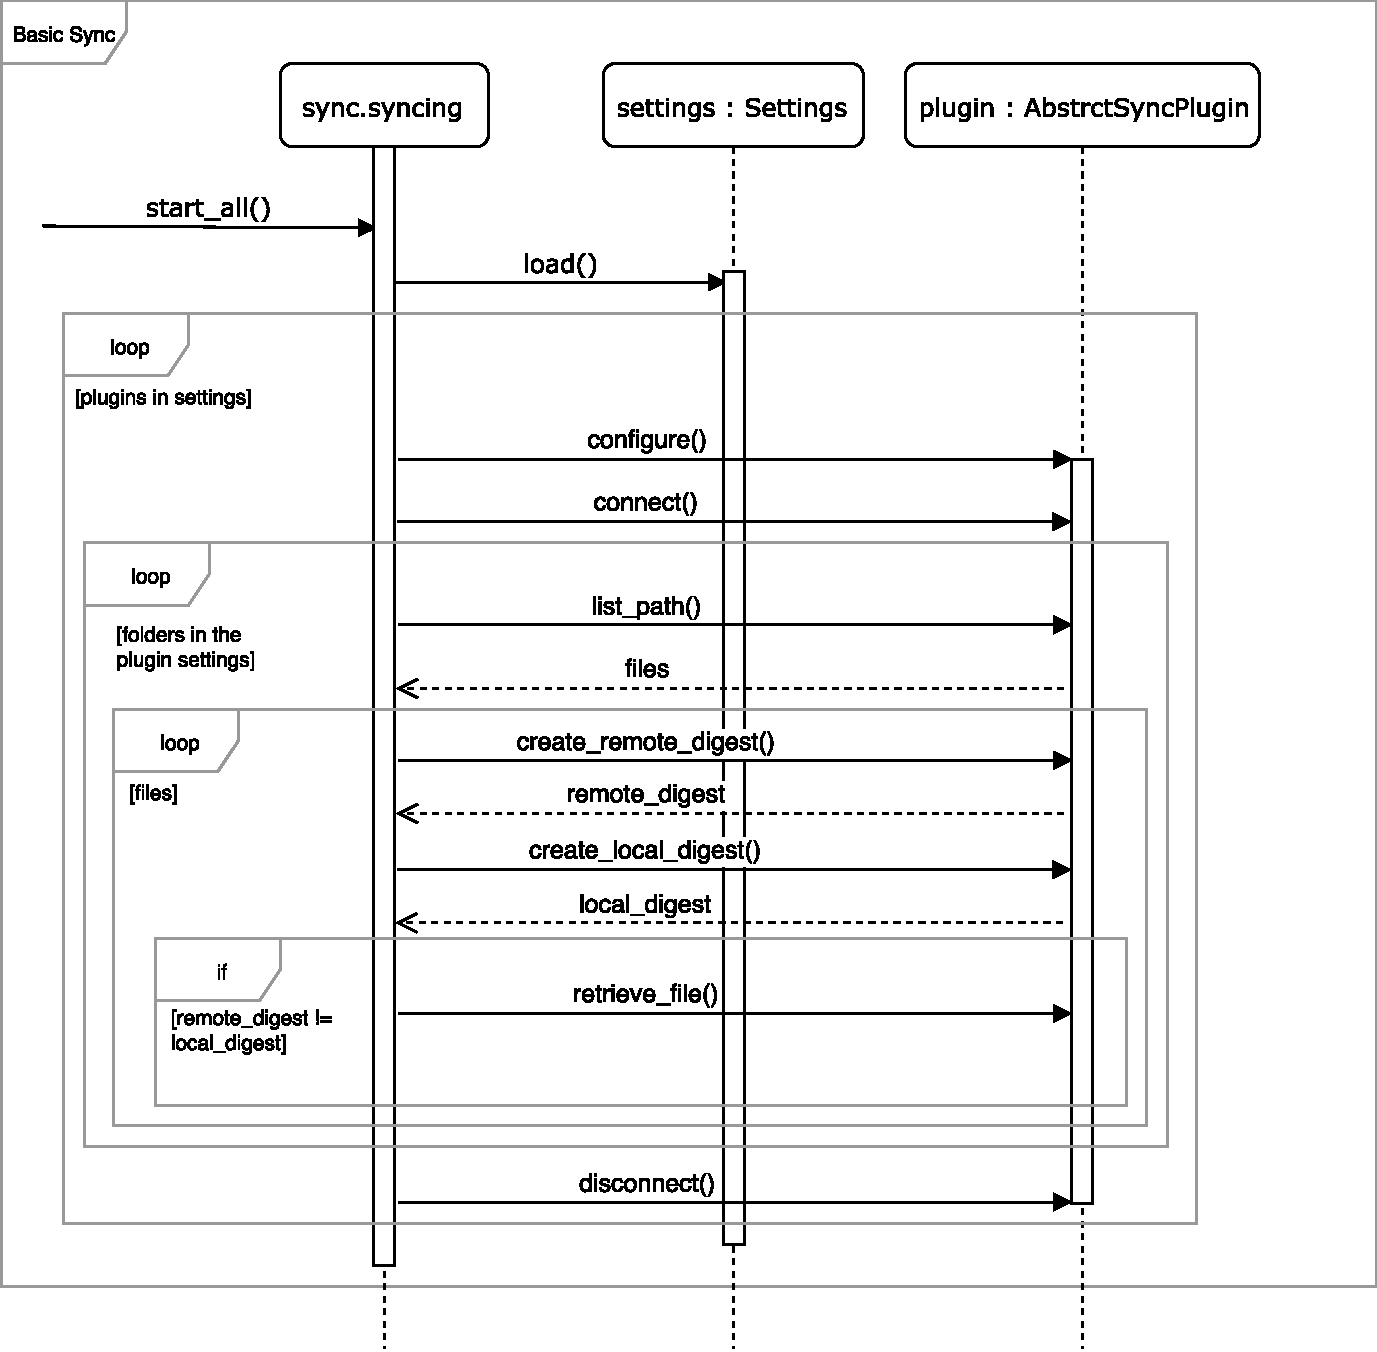
\includegraphics[width=40em]{./img/GrobesSequenzDiagramm.pdf}

\section{Prozesse und Threads}

% <Wenn mehrere Prozesse oder Threads eingesetzt werden wird hier beschrieben, wie diese ablaufen, miteinander funktionieren, Daten austauschen, sich synchronisieren, usw.>

Lösung für blockierend:

zwei separate Prozesse
zwei Threads
egal, es blockiert

Wir entscheiden:

Fürs Commandline-Interface wählen wir die Variante "egal, es blockiert".

Für GUI-Prototyp: 2 separate OS-Prozesse (GUI-Prozess, Kommand-Line-Interface).

Für die bessere GUI: Threads oder Python-Asynch (wahrscheinlich nicht mehr Teil des EngProj, wie im Projektplan festgelegt).

\section{Datenspeicherung}

% <Beschreibung mit Diagramm der Datenspeicherung (Datenmodell, z.B. Datenbank)>

Konfigurationsdatei: Wir wählen Plugin-Aufbau (Vorschlag  Nicolas Ganz ) und legen einen Konfig-Datei-Prototyp in EPJ-39 - Prototyp Konfiguration/Profile Au

iM Vordergrund steht die Verständlichkeit,d ass auch Studierende ausserhalb Informatik das File konfigurieren können.

FIXME Tabulatoren im Skript

\begin{verbatim}
root-dir: ~/Documents/HSR/semester_06

global-ignore:
	- Thumbs.db
	- .DS_Store

plugins:
	- name: skripte-server
		type: samba
		# server: svm-c213.hsr.ch
		# port: 445
		# share: skripte
		user: nganz
		# ...

sync:
	- name: Engineering-Projekt
		plugins:
			- plugin: skripte-server
		ignored:
			- SubDir
			- example.txt
		remote_dir: Informatik/Fachbereich/Engineering-Projekt/EPJ
		# local_dir: Engineering-Projekt
		# file downloaded: conflict-handling todo
\end{verbatim}


\end{document}
